\subsection{Limitations of each parameter}

\noindent
The problem of the RHF is that it does not differentiate between hydrides oriented within the ranges 0-40°, 40-65°, and 65-90° \cite{SIMON2021152817}. Thus, microstructures with different radial hydrides orientations can have the same $f_i$, which will lead to obtain the same value of RHF.

\noindent
The continuity factors do not differentiate some situations either. For example, the HCC is the same in the three situations illustrated in Figure \ref{fig:limitationhcc}, which certainly facilitate the cracking propagation to different extents. In Figure \ref{fig:limitationrhcf} it can be seen that two different situations entail the same value of RHCF and, on the contrary, Figure \ref{fig:sameconnectivity} shows how two equivalent situations may lead to different values of RHCF \cite{SIMON2021152817}.

\begin{figure}[h] %  figure placement: here, top, bottom, or page
    \centering
    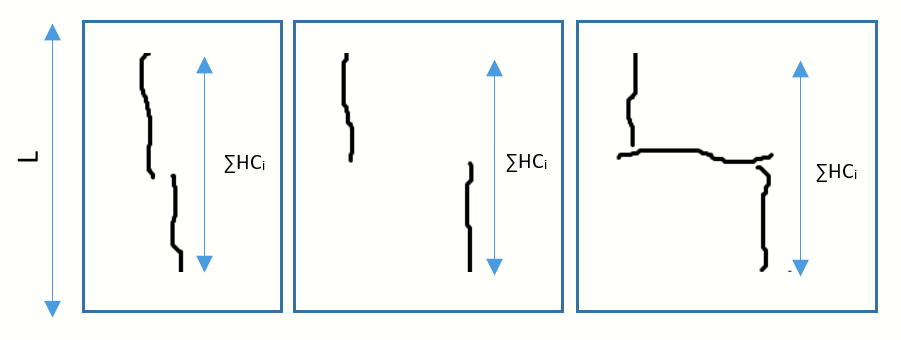
\includegraphics[width=4.5in]{Figures/3-Limitations/HCC comparison.png}
    \caption{Radial-oriented hydrides differently located but with the same HCC value.}
    \label{fig:limitationhcc}
\end{figure}

\begin{figure}[h] %  figure placement: here, top, bottom, or page
    \centering
    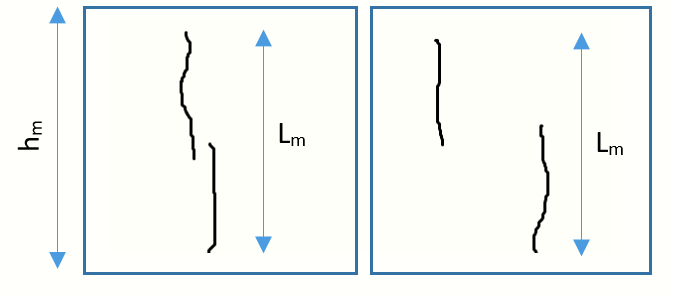
\includegraphics[width=4.5in]{Figures/3-Limitations/RHCF comparison 1.png}
    \caption{Radial-oriented hydrides with the same RHCF value but different connectivity.}
    \label{fig:limitationrhcf}
\end{figure}

\begin{figure}[h] %  figure placement: here, top, bottom, or page
    \centering
    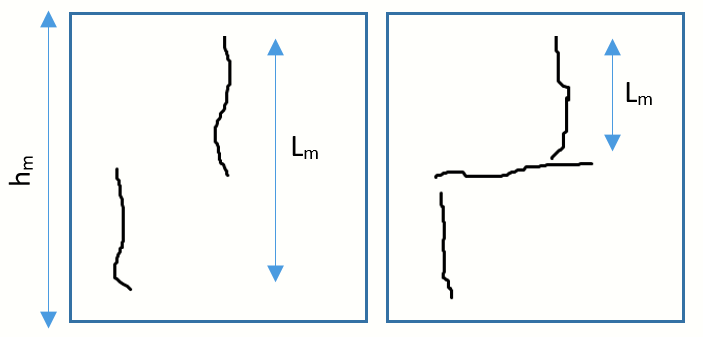
\includegraphics[width=4.5in]{Figures/3-Limitations/RHCF comparison 2.png}
    \caption{Radial-oriented hydrides with the different RHCF value but the same connectivity.}
    \label{fig:sameconnectivity}
\end{figure}
